\documentclass[a4paper,12pt]{article} % тип документа


% report, book


%%% Работа с русским языком % для pdfLatex
\usepackage{cmap}					% поиск в~PDF
\usepackage{mathtext} 				% русские буквы в~фомулах
\usepackage[T2A]{fontenc}			% кодировка
\usepackage[utf8]{inputenc}			% кодировка исходного текста
\usepackage[english,russian]{babel}	% локализация и переносы
\usepackage{indentfirst} 			% отступ 1 абзаца

%%% Работа с русским языком % для XeLatex
%\usepackage[english,russian]{babel}   %% загружает пакет многоязыковой вёрстки
%\usepackage{fontspec}      %% подготавливает загрузку шрифтов Open Type, True Type и др.
%\defaultfontfeatures{Ligatures={TeX},Renderer=Basic}  %% свойства шрифтов по умолчанию
%\setmainfont[Ligatures={TeX,Historic}]{Times New Roman} %% задаёт основной шрифт документа
%\setsansfont{Comic Sans MS}                    %% задаёт шрифт без засечек
%\setmonofont{Courier New}
%\usepackage{indentfirst}
%\frenchspacing

%%% Дополнительная работа с математикой
\usepackage{amsfonts,amssymb,amsthm,mathtools}
\usepackage{amsmath}
\usepackage{icomma} % "Умная" запятая: $0,2$~--- число, $0, 2$~--- перечисление
\usepackage{upgreek}

%%% Страница
\usepackage{extsizes} % Возможность сделать 14-й шрифт

%% Шрифты
\usepackage{euscript}	 % Шрифт Евклид
\usepackage{mathrsfs} % Красивый матшрифт

%% Свои команды
\DeclareMathOperator{\sgn}{\mathop{sgn}} % создание новой конанды \sgn (типо как \sin)
\usepackage{csquotes} % ещё одна штука для цитат
\newcommand{\pd}[2]{\ensuremath{\cfrac{\partial #1}{\partial #2}}} % частная производная
\newcommand{\abs}[1]{\ensuremath{\left|#1\right|}} % модуль
\renewcommand{\phi}{\ensuremath{\varphi}} % греческая фи
\newcommand{\pogk}[1]{\!\left(\cfrac{\sigma_{#1}}{#1}\right)^{\!\!\!2}\!} % для выражений для погрешности

% Ссылки
\usepackage{xcolor}
\usepackage{color} % подключить пакет color
% выбрать цвета
\definecolor{BlueGreen}{RGB}{49,152,255}
\definecolor{Violet}{RGB}{120,80,120}
% назначить цвета при подключении hyperref
\usepackage[unicode, colorlinks, urlcolor=blue, linkcolor=blue, pagecolor=blue, citecolor=blue]{hyperref} %синие ссылки
%\usepackage[unicode, colorlinks, urlcolor=black, linkcolor=black, pagecolor=black, citecolor=black]{hyperref} % для печати (отключить верхний!)
%\mathtoolsset{showonlyrefs=true} % Показывать номера только у тех формул, на которые есть \eqref{} в~тексте.


%% Перенос знаков в~формулах (по Львовскому)
\newcommand*{\hm}[1]{#1\nobreak\discretionary{}
	{\hbox{$\mathsurround=0pt #1$}}{}}

%%% Работа с картинками
\usepackage{graphicx}  % Для вставки рисунков
\graphicspath{{images/}{images2/}}  % папки с картинками
\setlength\fboxsep{3pt} % Отступ рамки \fbox{} от рисунка
\setlength\fboxrule{1pt} % Толщина линий рамки \fbox{}
\usepackage{wrapfig} % Обтекание рисунков и таблиц текстом
\usepackage{multicol}

%%% Работа с таблицами
\usepackage{array,tabularx,tabulary,booktabs} % Дополнительная работа с таблицами
\usepackage{longtable}  % Длинные таблицы
\usepackage{multirow} % Слияние строк в~таблице
\usepackage{caption}
\captionsetup{labelsep=period, labelfont=bf}

%%% Оформление
\usepackage{indentfirst} % Красная строка
\setlength{\parskip}{0.3cm} % отступы между абзацами

%%% Теоремы
\theoremstyle{plain} % Это стиль по умолчанию, его можно не переопределять.
\newtheorem{theorem}{Теорема}[section]
\newtheorem{proposition}[theorem]{Утверждение}

\theoremstyle{definition} % "Определение"
\newtheorem{definition}{Определение}[section]
\newtheorem{corollary}{Следствие}[theorem]
\newtheorem{problem}{Задача}[section]

\theoremstyle{remark} % "Примечание"
\newtheorem*{nonum}{Решение}
\newtheorem{zamech}{Замечание}[theorem]

%%% Правильные мат. символы для русского языка
\renewcommand{\epsilon}{\ensuremath{\varepsilon}}
\renewcommand{\phi}{\ensuremath{\varphi}}
\renewcommand{\kappa}{\ensuremath{\varkappa}}
\renewcommand{\le}{\ensuremath{\leqslant}}
\renewcommand{\leq}{\ensuremath{\leqslant}}
\renewcommand{\ge}{\ensuremath{\geqslant}}
\renewcommand{\geq}{\ensuremath{\geqslant}}
\renewcommand{\emptyset}{\varnothing}

\usepackage{graphicx}%Вставка картинок правильная
\usepackage{float}%"Плавающие" картинки
\usepackage{wrapfig}%Обтекание фигур (таблиц, картинок и прочего)

%%% Название разделов
\usepackage{titlesec}
\titlelabel{\thetitle.\quad} 

% новая команда \RNumb для вывода римских цифр
\newcommand{\RNumb}[1]{\uppercase\expandafter{\romannumeral #1\relax}}

% Цвета для гиперссылок
\definecolor{linkcolor}{HTML}{799B03} % цвет ссылок
\definecolor{urlcolor}{HTML}{799B03} % цвет гиперссылок
 
\hypersetup{pdfstartview=FitH,  linkcolor=linkcolor,urlcolor=urlcolor, colorlinks=true}

\usepackage[left=1.27cm,right=1.27cm,top=1.27cm,bottom=2cm]{geometry}

% нестандартные подписи 
\addto\captionsrussian{\def\chaptername{Глава}} 
\addto\captionsrussian{\def\contentsname{Содержание}} 
\addto\captionsrussian{\def\listfigurename{Список рисунков}} 
\addto\captionsrussian{\def\listtablename{Список таблиц}} 
\addto\captionsrussian{\def\abstractname{Аннотация}} 
\addto\captionsrussian{\def\refname{Список использованных источников}} 
\addto\captionsrussian{\def\indexname{Предметный указатель}} 
\addto\captionsrussian{\def\figurename{Рисунок}} 
\addto\captionsrussian{\def\tablename{Таблица}} 
\addto\captionsrussian{\def\partname{Часть}} 
\addto\captionsrussian{\def\appendixname{Приложение}}

%%% Органическая химия
\usepackage{chemfig}
\usepackage{xymtex}
%\usepackage{ochem}


%%% Фичи
\usepackage{cancel} % Диагональное и Х-зачёркивание
\usepackage{ulem} % Различные типы подчёркиваний


\begin{document} % начало документа
 
% НАЧАЛО ТИТУЛЬНОГО ЛИСТА
\begin{center}
\hfill \break
{МИНИСТЕРСТВО НАУКИ И ВЫСШЕГО ОБРАЗОВАНИЯ РОССИИ}\\
\footnotesize{ФЕДЕРАЛЬНОЕ ГОСУДАРСТВЕННОЕ АВТОНОМНОЕ ОБРАЗОВАТЕЛЬНОЕ}\\ 
\footnotesize{УЧРЕЖДЕНИЕ ВЫСШЕГО ОБРАЗОВАНИЯ}\\
\small{\textbf{«МОСКОВСКИЙ ФИЗИКО-ТЕХНИЧЕСКИЙ ИНСТИТУТ (НАЦИОНАЛЬНЫЙ ИССЛЕДОВАТЕЛЬСКИЙ УНИВЕРСИТЕТ)»}}\\
\hfill \break
\normalsize{Факультет биологической и медицинской физики}\\
\hfill \break

\hfill \break
\hfill \break
\hfill \break
\hfill\break
\hfill\break
\line(1,0){5030}\\[1mm]
\Large\textbf{{Лабораторная работа 3.1.1}}\\
\Large{Магнитометр}\\
\line(1,0){5030}\\[1mm]
\hfill \break
\hfill \break
\hfill \break
\hfill \break
\hfill \break
\hfill \break
\hfill \break
\end{center}
 
\begin{flushright}
{Выполнили:}

{Фитэль Алёна,}

{Попеску Полина}

{группа Б06-103}
\end{flushright}

\hfill \break
\hfill \break
\hfill \break
\hfill \break
\hfill \break
\hfill \break
\hfill \break
\begin{center} Долгопрудный,  \today \end{center}
\thispagestyle{empty} % выключаем отображение номера для этой страницы

% нестандартные подписи 
\addto\captionsrussian{\def\chaptername{Глава}} 
\addto\captionsrussian{\def\contentsname{Содержание}} 
\addto\captionsrussian{\def\listfigurename{Список рисунков}} 
\addto\captionsrussian{\def\listtablename{Список таблиц}} 
\addto\captionsrussian{\def\abstractname{Аннотация}} 
\addto\captionsrussian{\def\refname{Список использованных источников}} 
\addto\captionsrussian{\def\indexname{Предметный указатель}} 
\addto\captionsrussian{\def\figurename{Рисунок}} 
\addto\captionsrussian{\def\tablename{Таблица}} 
\addto\captionsrussian{\def\partname{Часть}} 
\addto\captionsrussian{\def\appendixname{Приложение}}
 
% КОНЕЦ ТИТУЛЬНОГО ЛИСТА

\newpage
\textbf{Цель работы:} определить горизонтальную составляющую магнитного поля Земли и установить количественное соотношение между
единицами электрического тока в системах СИ и СГС.

\textbf{Оборудование:} магнитометр, осветитель со шкалой, источник питания, вольтметр, электромагнитный переключатель, конденсатор, намагниченный стержень, прибор для определения периода
крутильных колебаний, секундомер, рулетка, штангенциркуль.

\section{Теоретическая справка}


\begin{wrapfigure}{l}{5cm}
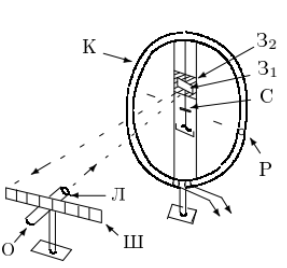
\includegraphics[scale=1]{magnet_scheme}
\caption{Схема магнитометра}
\end{wrapfigure}

В нашей установке с помощью
электромагнитного магнитометра измеряется горизонтальная составляющая земного магнитного поля и абсолютным образом определяется сила
тока по его магнитному действию.

\begin{wrapfigure}{r}{4cm}
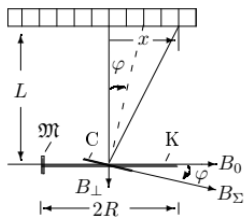
\includegraphics[scale=1]{magnet_angle}
\centering
\caption{{\small Схема измерения угла отклонения магнитной стрелки}}
\end{wrapfigure}
\textbf{Экспериментальная установка.}
Магнитометр (рис. 1) состоит из
нескольких последовательно соединённых круговых витков $K$, расположенных вертикально. В центре кольца $K$ на тонкой неупругой вертикальной нити подвешена короткая магнитная стрелка \textbf{$\rm C$}. Жёстко связанная со стрелкой крыльчатка погружена в масло и служит для демпфирования колебаний.

В отсутствие других магнитных полей стрелка располагается по направлению горизонтальной составляющей земного магнитного поля $\mathbf{B_0}$, т.е. лежит в плоскости магнитного меридиана.

Прибор настраивают с помощью световых зайчиков, отражённых
от двух зеркал: З$_1$, прикреплённого к стрелке (подвижный зайчик), и
З$_2$, расположенного в плоскости кольца $K$ и жёстко связанного с ним
(неподвижный зайчик). Оба зеркала освещаются одним и тем же осветителем $O$. Вращением кольца вокруг вертикальной оси можно совместить оба зайчика. При этом плоскость витков совпадает с плоскостью
магнитного меридиана.

При появлении дополнительного горизонтального магнитного поля $\mathbf{B_{\perp}}$ стрелка
$\rm C$ установится по равнодействующей обоих полей $\mathbf{B_{\Sigma}}$ (рис. 2). В нашей установке
дополнительное поле может быть создано
либо ферромагнитным стержнем, расположенным на кольце на его горизонтальном
диаметре ($\mathbf{B_1}$), либо током, проходящим
по кольцу ($\mathbf{B_2}$). В обоих случаях дополнительное поле можно считать однородным,
тк. размеры стрелки много меньше радиуса кольца.

Поле намагниченного стержня (точечного диполя) на перпендикуляре к нему:
\begin{equation}
	B_1=\dfrac{\mu_0}{4\pi }\dfrac{\mathfrak{M}}{R^3},
\end{equation}
поле в центре кольца с током по закону Био и Савара:
\begin{equation}
B_2=\dfrac{\mu_0 I}{2R}N.
\end{equation}
Здесь $\mathfrak{M}$ -- магнитный момент ферромагнитного стержня, $R$ — радиус
кольца, $N$ -- число витков в кольце, $I$ -- сила тока в единицах СИ (амперах).

Измерив угол отклонения стрелки $\phi$, можно связать поля $B_0$ и $B_\perp$ ($B_1$ или $B_2$):
\begin{equation}
B_{\perp}=B_0\cdot \tg \phi.
\end{equation}


\textsf{I. Определение горизонтальной составляющей магнитного поля Земли}

Для определения горизонтальной составляющей земного магнитного поля Во тонкий короткий намагниченный стержень устанавливается в отверстие Р на горизонтальном диаметре кольца (рис. 1). Измерив
тангенс угла отклонения стрелки
\begin{equation}
\tg \phi_1=\dfrac{x_1}{2L},
\end{equation} 
\noindent можно с помощью уравнений (1), (3) и (4) рассчитать поле $B_0$, если
исключить величину $\mathfrak{M}$ -- магнитный момент стержня.

Для исключения магнитного момента измерим период крутильных
колебаний стержня в поле Земли. Подвешенный горизонтально за середину на тонкой длинной нити сгержень в положении равновесия усгановится по полю Земли (упругость нити пренебрежимо мала). Если ось
стержня отклонить в горизонтальной плоскости от направления $B_0$ на
малый угол а, то под действием возвращающего механического момента
\[ M_{\text{мех}} = \mathfrak{M} B_0 \sin\alpha \approx \mathfrak{M} B_0 \alpha\]
стержень с моментом инерции $J$ в соответствии с уравнением
\[ J \dfrac{d^2 \alpha}{dt^2} + \mathfrak{M} B_0 \alpha =0   \]
будет совершать крутильные колебания с периодом

\begin{equation}
T=2\pi \sqrt{\dfrac{J}{\mathfrak{M}B_0}}.
\end{equation}
Момент инерции цилиндрического стержня относительно оси вращения
\begin{equation}
J=m\left(\dfrac{l^2}{12}+\dfrac{r^2}{4}\right)=\dfrac{ml^2}{12}\left[1+3\left(\dfrac{r}{l}\right)^2\right],
\end{equation}
где $m$ -- масса стержня, $l$ -- длина, а $r$ -- его радиус.


Таким образом, рассчитав момент инерции $J$ и измерив тангенс угла.
отклонения стрелки $\phi_1$ и период малых крутильных колебаний стержня $T$, можно с помощью формул (1), (3), (4) и (5) определить горизонтальную составляющую магнитного поля Земли:
\begin{equation}
B_0=\dfrac{2\pi}{TR}\sqrt{\dfrac{\mu_0 J L }{2\pi R x_1}}.
\end{equation}


\textsf{II. Определение электродинамической постоянной}

\begin{wrapfigure}{l}{5cm}
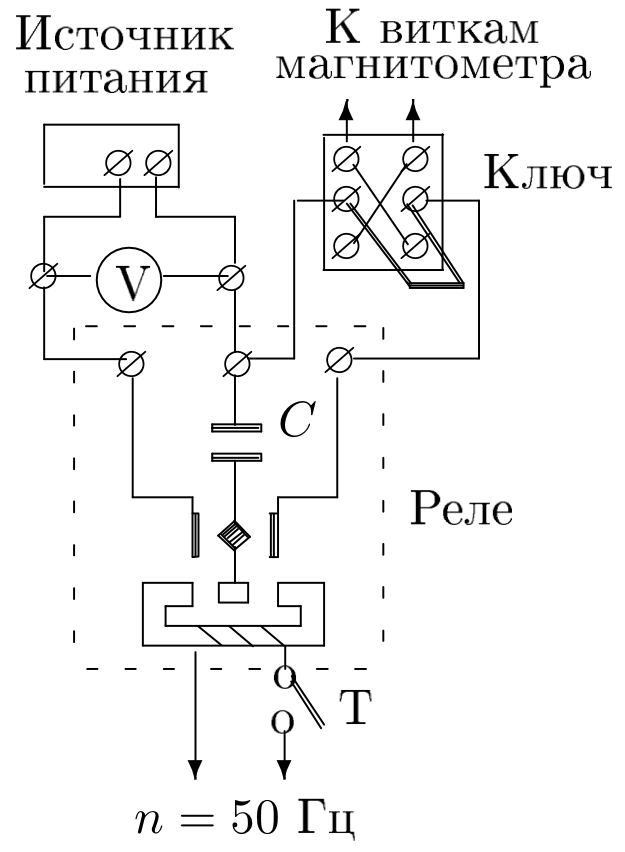
\includegraphics[scale=0.2]{pic.jpeg}
\caption{{\small Схема питания катушки магнитометра}}
\end{wrapfigure}

Для определения электродинамической постоянной с необходимо
провести независимые измерения одного и того же тока в разных системах: в СИ -- $I_{\text{СИ}}$ и в СГС -- $I_{\text{СГС}}$:

\begin{equation}
c=10\dfrac{\{I\}_{\text{СГС}}}{\{I\}_{\text{СИ}}}
\end{equation}

Пропуская ток через витки магнитометра, измеряют тангенс угла от
клонения стрелки ($\tg \phi_2 = \frac{x_2}{2L}$) и по формулам (2) и (3) рассчитывают величину
\begin{equation}
I_{\text{СИ}}=\dfrac{2B_0 R}{\mu_0 N}\tg \phi_2 = A\tg \phi_2.
\end{equation}
Величина А является постоянной прибора в данном месте земной поверхности.



Одновременно тот же ток измеряется в системе СГС (рис. 3). Если разрядить конденсатор ёмкости $C$, заря
женный до напряжения $U$, через витки, то через них протечёт заряд $q=CU$. Если $n$ раз в секунду после-
довательно заряжать конденсатор от источника и разряжать через витки,
то через них за секунду протечёт заряд $CUn$. Средний ток, прошедший
через витки, равен при этом
\begin{equation}
I_{\text{СГС}}=CUn.
\end{equation}




\section{Обработка результатов}

\subsection{Определение горизонтальной составляющей магнитного поля Земли}
\begin{large}
\textbf{Параметры установки:}
\begin{itemize}
\item Отклонение $x_1 = 3.5\pm 0,1~\text{см}, \tilde x_1 = 2.8\pm 0,1~\text{см} $
\item Расстояние от шкалы до зеркала $L=111\pm 1~\text{см}.$
\item Радиус кольца $R=20,0\pm 0,1$ см
\end{itemize}


\textbf{Параметры стержня:}
\begin{itemize}
\item $m=4,350\pm 0,001$ г;
\item $d = 4,00\pm 0,01~\text{мм} \Rightarrow r=2,000\pm 0,005$ мм;
\item $\l = 45,00\pm 0,01$ мм.
\end{itemize}


За $132.1$ cекунд произошло 10 колебаний, следовательно, период $T=13.2\pm 0,3$ секунд.

\noindent По формуле   
\[J=\dfrac{ml^2}{12}\left[1+3\left(\dfrac{r}{l}\right)^2\right]\]
найдём момент инерции стержня, $J= 7,38\cdot 10^{-7}~\text{кг}\cdot \text{м}^2$. Погрешность $\sigma_J = 4,6\cdot 10^{-9}~\text{кг}\cdot \text{м}^2.$

\noindent Найдём величину $B_0$ горизонтальной составляющей магнитного поля Земли по формуле:
\[B_0=\dfrac{2\pi}{TR}\sqrt{\dfrac{\mu_0 J L }{2\pi R x_1}}=(115\pm4)\cdot 10^{-7}~\text{Тл}\]


\subsection{Определение электродинамической постоянной}

\textbf{Параметры установки:}
\item Расстояние от шкалы до зеркала $L=111\pm 1~\text{см}.$
\begin{itemize}
\item Рабочее напряжение $U=98$ В;
\item Электроёмкость конденсатора $C=9\cdot 10^5~\text{см}\pm 2\%=1,896~\text{мкФ}$;
\item N = 44 витка;
\item Радиус кольца $R=20,0\pm 0,1$ см
\item Частота $n=50$ Гц.
\end{itemize}

При включении электровибратора отклонение <<зайчика>> вправо: $A_1=3.5$ см, отклонение влево: $A_2=2.8$ см $\Rightarrow$ cреднее отклонение $x_2=(A_1+A_2)/2=3.2$ см. Тогда по формуле (9):
\[I_{\text{СИ}}=\dfrac{2B_0R}{\mu_0 N}\dfrac{x_2}{2L}=1.2\cdot 10^{-3}~A;~~~\sigma I_{\text{СИ}}=0.3\cdot 10^{-3}~A.\]

$I_\text{СГС}$ найдём по формуле (10):
\[I_\text{СГС}=CUn=147\cdot 10^5~\text{ед. СГСЭ};~~~\sigma I_{\text{СГС}}=3\cdot 10^{5} \text{ед. СГСЭ}.\] 

Тогда найдём $c:$
\[c=10\dfrac{\{I\}_\text{СГС}}{\{I\}_{\text{СИ}}}=(11\pm3)\cdot 10^{10}~\dfrac{\text{ед. СГСЭ}}{A};\]


\section{Вывод}
В ходе работы была определенна горизонтальная составляющая магнитного поля Земли ($B_0=(115\pm4)\cdot 10^{-7}~\text{Тл}$) и было установлено количественное соотношение между
единицами электрического тока в системах СИ и СГС, $c=(11\pm3)\cdot 10^{10}~\dfrac{\text{ед. СГСЭ}}{A}.$ Несовпадение полученной величины с табличым значением константы $c=3\cdot 10^{10}~\dfrac{\text{ед. СГСЭ}}{A}$, может быть связано с отличием значения горизонтальной составляющей магнитного поля Земли, полученной в первой части работы, с той, которая была во второй части, вследствие влияния соседних установок и электронных устройств на итоговое горизонтальное поле.

\end{large}





\end{document}



